% Options for packages loaded elsewhere
\PassOptionsToPackage{unicode}{hyperref}
\PassOptionsToPackage{hyphens}{url}
%
\documentclass[
]{book}
\usepackage{amsmath,amssymb}
\usepackage{iftex}
\ifPDFTeX
  \usepackage[T1]{fontenc}
  \usepackage[utf8]{inputenc}
  \usepackage{textcomp} % provide euro and other symbols
\else % if luatex or xetex
  \usepackage{unicode-math} % this also loads fontspec
  \defaultfontfeatures{Scale=MatchLowercase}
  \defaultfontfeatures[\rmfamily]{Ligatures=TeX,Scale=1}
\fi
\usepackage{lmodern}
\ifPDFTeX\else
  % xetex/luatex font selection
\fi
% Use upquote if available, for straight quotes in verbatim environments
\IfFileExists{upquote.sty}{\usepackage{upquote}}{}
\IfFileExists{microtype.sty}{% use microtype if available
  \usepackage[]{microtype}
  \UseMicrotypeSet[protrusion]{basicmath} % disable protrusion for tt fonts
}{}
\makeatletter
\@ifundefined{KOMAClassName}{% if non-KOMA class
  \IfFileExists{parskip.sty}{%
    \usepackage{parskip}
  }{% else
    \setlength{\parindent}{0pt}
    \setlength{\parskip}{6pt plus 2pt minus 1pt}}
}{% if KOMA class
  \KOMAoptions{parskip=half}}
\makeatother
\usepackage{xcolor}
\usepackage{color}
\usepackage{fancyvrb}
\newcommand{\VerbBar}{|}
\newcommand{\VERB}{\Verb[commandchars=\\\{\}]}
\DefineVerbatimEnvironment{Highlighting}{Verbatim}{commandchars=\\\{\}}
% Add ',fontsize=\small' for more characters per line
\usepackage{framed}
\definecolor{shadecolor}{RGB}{248,248,248}
\newenvironment{Shaded}{\begin{snugshade}}{\end{snugshade}}
\newcommand{\AlertTok}[1]{\textcolor[rgb]{0.94,0.16,0.16}{#1}}
\newcommand{\AnnotationTok}[1]{\textcolor[rgb]{0.56,0.35,0.01}{\textbf{\textit{#1}}}}
\newcommand{\AttributeTok}[1]{\textcolor[rgb]{0.13,0.29,0.53}{#1}}
\newcommand{\BaseNTok}[1]{\textcolor[rgb]{0.00,0.00,0.81}{#1}}
\newcommand{\BuiltInTok}[1]{#1}
\newcommand{\CharTok}[1]{\textcolor[rgb]{0.31,0.60,0.02}{#1}}
\newcommand{\CommentTok}[1]{\textcolor[rgb]{0.56,0.35,0.01}{\textit{#1}}}
\newcommand{\CommentVarTok}[1]{\textcolor[rgb]{0.56,0.35,0.01}{\textbf{\textit{#1}}}}
\newcommand{\ConstantTok}[1]{\textcolor[rgb]{0.56,0.35,0.01}{#1}}
\newcommand{\ControlFlowTok}[1]{\textcolor[rgb]{0.13,0.29,0.53}{\textbf{#1}}}
\newcommand{\DataTypeTok}[1]{\textcolor[rgb]{0.13,0.29,0.53}{#1}}
\newcommand{\DecValTok}[1]{\textcolor[rgb]{0.00,0.00,0.81}{#1}}
\newcommand{\DocumentationTok}[1]{\textcolor[rgb]{0.56,0.35,0.01}{\textbf{\textit{#1}}}}
\newcommand{\ErrorTok}[1]{\textcolor[rgb]{0.64,0.00,0.00}{\textbf{#1}}}
\newcommand{\ExtensionTok}[1]{#1}
\newcommand{\FloatTok}[1]{\textcolor[rgb]{0.00,0.00,0.81}{#1}}
\newcommand{\FunctionTok}[1]{\textcolor[rgb]{0.13,0.29,0.53}{\textbf{#1}}}
\newcommand{\ImportTok}[1]{#1}
\newcommand{\InformationTok}[1]{\textcolor[rgb]{0.56,0.35,0.01}{\textbf{\textit{#1}}}}
\newcommand{\KeywordTok}[1]{\textcolor[rgb]{0.13,0.29,0.53}{\textbf{#1}}}
\newcommand{\NormalTok}[1]{#1}
\newcommand{\OperatorTok}[1]{\textcolor[rgb]{0.81,0.36,0.00}{\textbf{#1}}}
\newcommand{\OtherTok}[1]{\textcolor[rgb]{0.56,0.35,0.01}{#1}}
\newcommand{\PreprocessorTok}[1]{\textcolor[rgb]{0.56,0.35,0.01}{\textit{#1}}}
\newcommand{\RegionMarkerTok}[1]{#1}
\newcommand{\SpecialCharTok}[1]{\textcolor[rgb]{0.81,0.36,0.00}{\textbf{#1}}}
\newcommand{\SpecialStringTok}[1]{\textcolor[rgb]{0.31,0.60,0.02}{#1}}
\newcommand{\StringTok}[1]{\textcolor[rgb]{0.31,0.60,0.02}{#1}}
\newcommand{\VariableTok}[1]{\textcolor[rgb]{0.00,0.00,0.00}{#1}}
\newcommand{\VerbatimStringTok}[1]{\textcolor[rgb]{0.31,0.60,0.02}{#1}}
\newcommand{\WarningTok}[1]{\textcolor[rgb]{0.56,0.35,0.01}{\textbf{\textit{#1}}}}
\usepackage{longtable,booktabs,array}
\usepackage{calc} % for calculating minipage widths
% Correct order of tables after \paragraph or \subparagraph
\usepackage{etoolbox}
\makeatletter
\patchcmd\longtable{\par}{\if@noskipsec\mbox{}\fi\par}{}{}
\makeatother
% Allow footnotes in longtable head/foot
\IfFileExists{footnotehyper.sty}{\usepackage{footnotehyper}}{\usepackage{footnote}}
\makesavenoteenv{longtable}
\usepackage{graphicx}
\makeatletter
\def\maxwidth{\ifdim\Gin@nat@width>\linewidth\linewidth\else\Gin@nat@width\fi}
\def\maxheight{\ifdim\Gin@nat@height>\textheight\textheight\else\Gin@nat@height\fi}
\makeatother
% Scale images if necessary, so that they will not overflow the page
% margins by default, and it is still possible to overwrite the defaults
% using explicit options in \includegraphics[width, height, ...]{}
\setkeys{Gin}{width=\maxwidth,height=\maxheight,keepaspectratio}
% Set default figure placement to htbp
\makeatletter
\def\fps@figure{htbp}
\makeatother
\setlength{\emergencystretch}{3em} % prevent overfull lines
\providecommand{\tightlist}{%
  \setlength{\itemsep}{0pt}\setlength{\parskip}{0pt}}
\setcounter{secnumdepth}{5}
\usepackage{booktabs}
\ifLuaTeX
  \usepackage{selnolig}  % disable illegal ligatures
\fi
\usepackage[]{natbib}
\bibliographystyle{plainnat}
\IfFileExists{bookmark.sty}{\usepackage{bookmark}}{\usepackage{hyperref}}
\IfFileExists{xurl.sty}{\usepackage{xurl}}{} % add URL line breaks if available
\urlstyle{same}
\hypersetup{
  pdftitle={Manifolds},
  pdfauthor={Ashan Jayamal \& Nalamudu Samarasinghe},
  hidelinks,
  pdfcreator={LaTeX via pandoc}}

\title{Manifolds}
\author{Ashan Jayamal \& Nalamudu Samarasinghe}
\date{2024-03-05}

\usepackage{amsthm}
\newtheorem{theorem}{Theorem}[chapter]
\newtheorem{lemma}{Lemma}[chapter]
\newtheorem{corollary}{Corollary}[chapter]
\newtheorem{proposition}{Proposition}[chapter]
\newtheorem{conjecture}{Conjecture}[chapter]
\theoremstyle{definition}
\newtheorem{definition}{Definition}[chapter]
\theoremstyle{definition}
\newtheorem{example}{Example}[chapter]
\theoremstyle{definition}
\newtheorem{exercise}{Exercise}[chapter]
\theoremstyle{definition}
\newtheorem{hypothesis}{Hypothesis}[chapter]
\theoremstyle{remark}
\newtheorem*{remark}{Remark}
\newtheorem*{solution}{Solution}
\begin{document}
\maketitle

{
\setcounter{tocdepth}{1}
\tableofcontents
}
\hypertarget{basic-theroms-and-definitions}{%
\chapter{Basic Theroms and Definitions}\label{basic-theroms-and-definitions}}

\begin{definition}[Topology]
\protect\hypertarget{def:Top}{}\label{def:Top}A topology on a set \(X\) is a collection \(\mathcal{T}\) of subsets of \(X\) such that

\textbf{(T1)} \(\phi\) and \(X\) are in \(\mathcal{T}\);

\textbf{(T2)} Any union of subsets in \(\mathcal{T}\) is in \(\mathcal{T}\);

\textbf{(T3)} The finite intersection of subsets in \(\mathcal{T}\) is in \(\mathcal{T}\).
\end{definition}

A set \(X\) with a topology \(\mathcal{T}\) is called a topological space. Denoted by \((X,\mathcal{T})\). An element of \(\mathcal{T}\) is called an open set.

\begin{definition}
\protect\hypertarget{def:unnamed-chunk-1}{}\label{def:unnamed-chunk-1}A subset \(U \subset M\) is referred to as open in \(M\) if \(U \in \mathcal{T}\). A subset \(A \subset M\) is termed closed if \(M \setminus A \in \mathcal{T}\).
\end{definition}

\begin{definition}[Continuity]
\protect\hypertarget{def:unnamed-chunk-2}{}\label{def:unnamed-chunk-2}If both \((M, \mathcal{T}_M)\) and \((N, \mathcal{T}_N)\) are topological spaces, a map \(f : M \rightarrow N\) is termed continuous if \[f^{-1}(V) \in \mathcal{T}_M \text{ for all } V \in \mathcal{T}_N\].
In other words, the preimages of open sets must be open.
\end{definition}

\begin{definition}[Homemorphism]
\protect\hypertarget{def:unnamed-chunk-3}{}\label{def:unnamed-chunk-3}A map \(f : M \rightarrow N\) between two topological spaces is called homemorphism if it has following propoties.
- \(f\) is a bijection,
- \(f\) is continuous,
- the inverse function \(f^{-1}\) is continuous.

Two topological spaces \(M\) and \(N\) are called homeomorphic if there exists a homeomorphism between them.
\end{definition}

\begin{definition}[Hausdorff Space]
\protect\hypertarget{def:unnamed-chunk-4}{}\label{def:unnamed-chunk-4}A topological space \((X,\mathcal{T})\) is called a Hausdorff space if\\
\textbf{(H1)} \(\forall x,y \in X\) such that \(x \neq y\), \(\exists U_x, U_y \in \mathcal{T}\) such that \(x \in U_x\), \(y \in U_y\), and \(U_x \cap U_y = \emptyset\).

i.e., for every pair of distinct points \(x, y\) in \(X\), there are disjoint neighborhoods \(U_x\) and \(U_y\) of \(x\) and \(y\) respectively.
\end{definition}

\begin{figure}
\centering
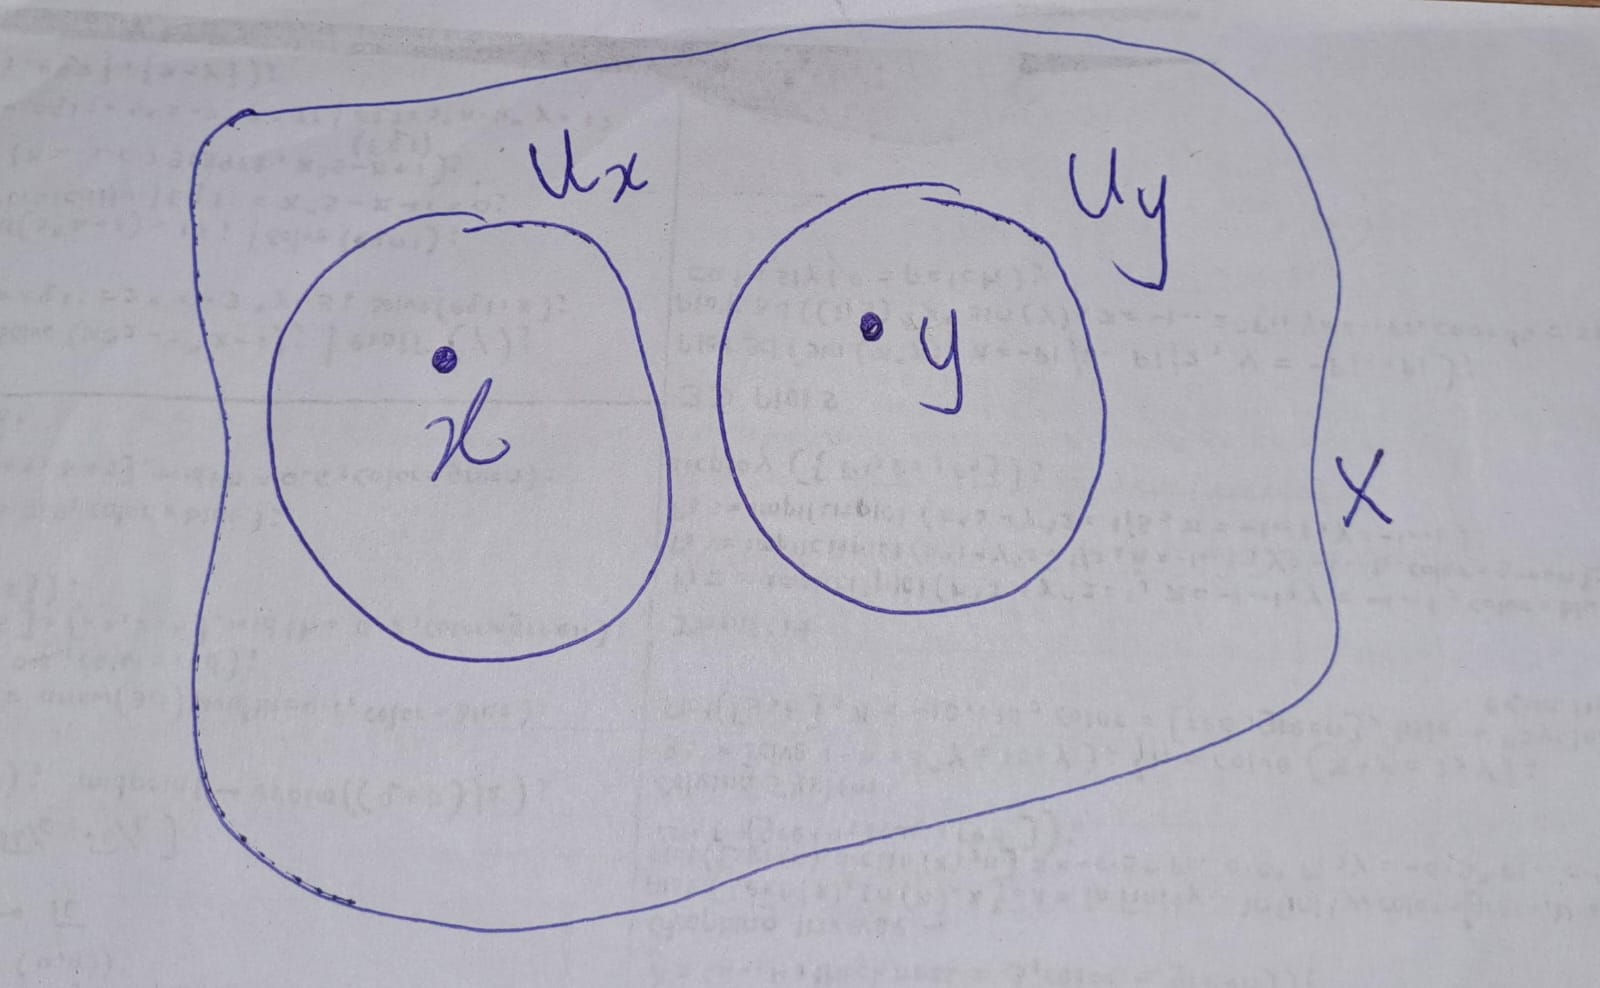
\includegraphics{figures/ch1/fig01.jpg}
\caption{\label{fig:fig01}\(~\)}
\end{figure}

\begin{Shaded}
\begin{Highlighting}[]
\NormalTok{A space $X$ is said to have a **countable basis at the point $x$** if there is a countable collection $\textbackslash{}\{U\_n\textbackslash{}\}\_\{n\textbackslash{}in\textbackslash{}mathbb\{Z\}\^{}+\}$ of neighborhoods of $x$ such that any neighborhood $U$ of $x$ contains at least one of the sets $U\_n$. A space $X$ that has a countable basis at each of its points is said to satisfy the first countability axiom.}
\end{Highlighting}
\end{Shaded}

\hypertarget{manifolds}{%
\chapter{Manifolds}\label{manifolds}}

\hypertarget{topological-manifolds}{%
\section{Topological Manifolds}\label{topological-manifolds}}

  \bibliography{book.bib,packages.bib}

\end{document}
